\newpage
\chapter{Операторы физических величин и их собственные значения}

\par Пусть у нас имеется несколько классических приборов, измеряющих некую физическую величину. Обозначим её \textit{f}, каждой такой величине ставится в соответствие оператор $\hat{f}$, который может действовать на волновую функцию $\psi$. Процесс измерения заключается в том, что классический прибор и частица приходят во взаимодействие друг с другом, в результате чего прибор переходит из начального в некоторое другое состояние, и по этому состоянию мы судим о состоянии частицы. Описание состояний прибора осуществляется квазиклассическими волновыми функциями. Тогда в результате измерения величины \textit{f} получим набор собственных значений $f_n$:
$$ \hat{f} \psi _n (\vec{r}, t) = f_n \psi_n $$
\par С другой стороны, на вход прибора совершенно не обязательно приходит собственная функция, может быть и суперпозиция с некоторыми коэффициентами разложения, т.е. с прибора мы снимаем среднее значение величины \textit{f}, а значит в каждом конкретном измерении получаем какое-то одно $f_n$, не меняя условий эксперимента и возвращая частицу к начальному состоянию, повторяем многократно, а затем усредняем результат:
$$ \overline{f} = \int \psi ^* \hat{f} \psi d^3r =  \int \psi ^* \hat{f} \psi dq$$
\par Условие нормировки $\int |\psi|^2 dq = 1$ (т.к. речь идет о вероятности найти частицу хоть где-то, о классе функций). Но так хорошо работать только с дискретным спектром собственных значений $f_n$, т.к. функция хорошо локализована в пространстве и интеграл существует. С непрерывным спектром оператора есть некоторые тонкости, о которых пока не будем  говорить. Можно себя успокаивать так: любую частицу можем закрыть в ящике, где нормировка может быть осуществлена.
\par Конкретизируем аксиоматику (написать уравнение на волновую функцию, установить правила определения операторов физ. величин). Получить операторы физических величин нельзя, но можно ввести их, учитывая, что в конкретных пределах не должно быть отличия от классики. Начнем с вида волновой функции.

\begin{wrapfigure}[8]{l}{0.25\linewidth} 
\vspace{-2ex}
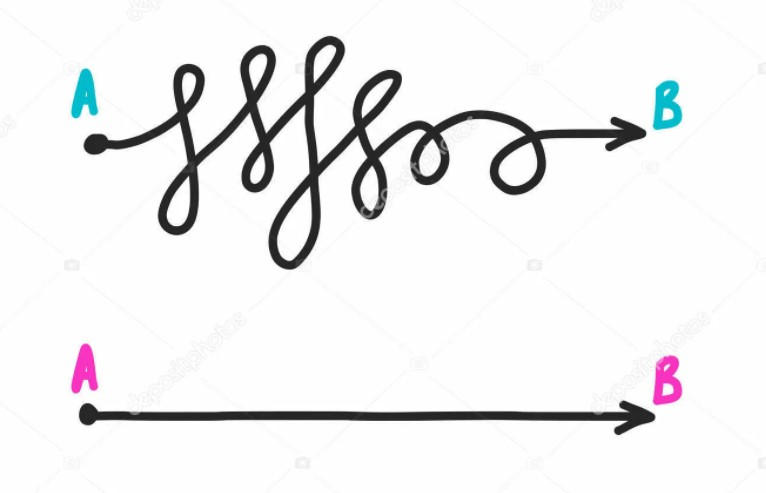
\includegraphics[width=1.1\linewidth]{pictures/5.1.jpg}
\caption{Иллюстрация к принципу Ферма}
\end{wrapfigure}

\par В качестве классического предела для волновой функции рассмотрим $\psi \sim e^{i \frac{S}{\hbar}}$, где \textit{S} - действие, эйконал. Все это представление должно срастить с уравнениями Ньютона, т.е. с экстремумом действия \textit{S}. Для света длину оптического пути можно найти из принципа Ферма: свет выбирает из множества путей между двумя точками тот путь, который потребует наименьшего времени (по лучу). А значит, требуется найти минимум функционала $ S = \int_{A}^{B} n dl$, где $n = \sqrt{\varepsilon}$ - показатель преломления. Как это получить из уравнений Максвелла? $ \frac{\varepsilon}{c^2} \frac{\partial ^2 }{\partial t ^2} \vec{A} = \underbrace{- \frac{4 \pi}{c} \vec{j}}_{\text{какие-то источники}} $. Векторный потенциал с полями связаны следующим образом:
$$\vec{B} = rot \vec{A} $$
$$ \vec{E} = - \frac{1}{c} \frac{\partial \vec{A}}{\partial t} - \nabla \varphi$$
\par То, о чем мы говорим - приближение, которое верно при определенных условиях (ведь то, что свет пойдет по лучу - тоже приближение, не учитывающее дифракцию и интерференцию). Пусть \textit{n} однородно, тогда ищем решения уравнения Максвелла в виде $e^{-iwt +i \vec{k} \vec{r}}$. Свет распространяется вдоль вектора $\vec{k}$, это и есть лучи из принципа Ферма. Можем попробовать искать поля $\vec{E}, \vec{B} \sim \vec{a} \cdot e^{i \varphi}$:
$$ \frac{\partial \varphi}{\partial t} = -w $$
$$ \frac{\partial \varphi}{\partial \vec{r}} = \vec{k} (\vec{r}) $$
\par Откуда $$ \varphi = -wt + \frac{\epsilon w}{c} \varphi_1 $$
$$ (\nabla \varphi _1)^2 =n^2 (x,y,z) \Longrightarrow \varphi_1 = \int n dl $$
\par Где $\varphi_1$ играет роль эйконала, а интегрирование ведется вдоль луча. Линии градиента можем воспринимать как эти лучи, они имеют смысл локального вектора $\vec{k}$. $rot(\nabla \varphi_1)=0 \longrightarrow $ получим решение, которое работает, если масштаб изменения свойств среды $L(n) >> \lambda$. (В лучевой $\lambda \approx 0$, а масштабы искривления много больше) Приближение геметрической оптики здесь называется \textit{эйкональным приближением}.

\begin{table}[h]
\centering
\begin{tabular}[c]{|c|c|}
\hline 
Оптика & Хотим аналог в квантах \\ \hline 
Эйконал S & Действие S \\
$\varphi, \vec{A} \sim e^{iS} $ & $\psi \sim e^{i \frac{S}{\hbar}}$ \\
лучи & траектории по Ньютону \\
принцип Ферма & принцип Мопертюи \\
$dS =-w dt + \frac{w}{c} \vec{k} d\vec{l}$ & $dS=-Hdt+ \sum_{i}p_idq_i$ \\
\hline
\end{tabular}
\end{table}
\par Из теоретической механики знаем, что для нахождения минимума функционала действия, нужно проварьировать его и приравнять первую вариацию к нулю:
$$\delta S = \sum_{i} \frac{\partial L}{\partial \dot{q_i}} \delta q_i \bigg|_{t_1}^{t} + \sum_{i} \int_{t_i}^{t} \underbrace{ \bigg( \frac{\partial L}{\partial q_i} - \frac{d}{dt} \frac{\partial L}{\partial \dot{q_i}} \bigg) }_{\text{для классической механики ноль}} \delta q_i dt $$
$$ \delta q_i(t_1)=0 \Longrightarrow \delta S = \sum_{i} p_i \delta q_i $$
$$ \frac{dS}{dt} = \frac{\partial S}{\partial t} +\sum \frac{\partial S}{\partial q_i} \dot{q_i} = \frac{\partial S}{\partial t}+ \sum p_i \dot{q_i} \Longrightarrow \frac{\partial S}{\partial t} = L -  \sum_{i} p_i \dot{q_i}= -H  $$
\par По аналогии с оптикой хочется, чтоб выполнялся закон сохранения энергии $E=H \Longrightarrow S = \underbrace{\int \sum p_i dq_i}_{\text{укороченное действие }S_0} - E(t-t_0)$. Для материальной точки в 3D, например, $p=\sqrt{2m(E-U)}$, $$S_0 = \int \vec{p}d \vec{r}=\int \sqrt{2m(E-U(\vec{r}))} dl $$
\par Назовем подынтегральное выражение показателем преломления n и получим аналог принципа Ферма - \textit{принцип Мопертюи}.
\par В уравнении на $\psi$ желательна некая линейность (ради выполнения принципа суперпозиции), рассмотрим:
$$ \frac{\partial \psi}{\partial t} =\frac{\partial}{\partial t} ( e^{i \frac{S}{\hbar}} ) = \frac{i}{\hbar} \frac{\partial S}{\partial t} \Psi =  \frac{i}{\hbar} (-H) \psi$$
\par Так называемое уравнение Шрёдингера
$$ i \hbar \frac{\partial \psi}{\partial t} = H \psi $$
\par Теперь отказываемся от идеи $\psi \sim e^{\frac{iS}{\hbar}}$, запишем оператор Гамильтониана $$\hat{H} = \frac{\hat{\vec{p}}^2}{2m}+U(\hat{\vec{r}})$$
\par Осталось определить, что есть оператор импульса и координаты и  \colorbox{orange}{как они действуют на $\psi$.}
$$ \hat{\vec{p}} \psi = \nabla S \psi  \Longrightarrow \hat{\vec{p}} = -i \hbar \nabla  $$
\par Уравнение без источника, значит, нужны условия на $\psi$:  $\psi \ne 0 $ + условие нормировки $\int |\psi|^2 d^3r = 1$. Продифференцируем последнее соотношение по времени:
$$ \int dq (\dot{\psi} \psi^{*} +\psi \dot{\psi^{*}}) = \int dq ( \psi^{*} \frac{\hat{H}}{i \hbar} \psi - \psi \frac{\hat{H^*}}{i \hbar} \psi^*) =\frac{1}{i \hbar} \int \psi^*\hat{H} \psi dq - \underbrace{\frac{1}{i \hbar} \int \psi^*\hat{\widetilde{H}} \psi dq}_{\text{здесь поменяли местами } \psi^* \text{ и }\psi} = 0 $$
\par Здесь $\hat{\widetilde{H}}$ - транспонированный оператор, $\hat{\widetilde{H}}^* = \hat{H}^+$ - оператор, эрмитово сопряженный исходному. Для выполнения верхнего равенства требуем эрмитовость оператора гамильтониана $\hat{H}=\hat{H}^+$ ($\forall \psi$). 
\par \textit{Небольшое отступление. Все ли операторы физических величин эрмитовы? Рассмотрим оператор импульса} $\hat{\vec{p}} = -i \hbar \nabla$: определению соответствует $$ \int \psi_1 \hat{\vec{p}} \psi_2 dq = -i \hbar \int (\underbrace{\nabla (\psi_1 \psi_2)}_{\text{Хотим ноль на }\infty} - \psi_2 \nabla \psi_1) dq = \int \psi_2 (i \hbar \nabla)\psi_1 dq \Longrightarrow \hat{p}^т=-\hat{p} $$
$$ \hat{p}^+ = -\hat{p}^* = \hat{p} \text{- эрмитов}$$
\par \textit{Для вычисления любой величины требуется найти среднее: $\overline{f}=\int \psi^* \hat{f} \psi dq$. Показания классического прибора должны быть действительными} $ \overline{f} \in \mathbb{R}$. 
$$ \overline{f^*}= \int \psi \hat{f^*} \psi^* dq = \int \psi^* \hat{f^+} \psi dq$$
\par \textit{Это выполняется $\forall \psi$, следовательно, $\hat{f^+} = \hat{f}$.}

\par Итак, хотим найти собственные функции оператора импульса $ \hat{\vec{p}} \psi_p = \vec{p} \psi _p $, фактически, мы раскладываем $\psi_p$-функцию по базису из собственных функций оператора $\hat{\vec{p}}$, получаем $\psi_p \sim e^{\frac{i\vec{p}\vec{r}}{\hbar}}$ - плоские волны.
\par Оператор координаты - это домножение на нее: $\hat{x} \psi = x_0 \psi$, собственной функцией данного оператора является $\delta$-функция. (Вообще именно поэтому мы не можем перейти от одного к другому, от $\delta$-функции к плоским волнам: $[\hat{x}\hat{p}]=i\hbar$)
\par Теперь рассмотрим оператор параллельного переноса $\hat{T}_{\vec{a}} \psi (\vec{r}) = \psi ( \vec{r} + \vec{a} )$. Для этого разложим $\psi (\vec{r}+\vec{a})$ в ряд Тейлора и заменим производную по r на известное нам действие оператора $\hat{\vec{p}}$ с соотвествующими коэффициентами:
$$\psi (\vec{r}+\vec{a}) = \psi (\vec{r}) + \vec{a} \frac{\partial}{\partial r} \psi + ... = (1+\frac{i}{\hbar}(\vec{a}\hat{\vec{r}}) + \frac{1}{2}(\frac{i}{\hbar}(\vec{a}\hat{\vec{r}})^2) +...)\psi $$
\par Получим $$\hat{T}_{\vec{a}} = e^{\frac{i}{\hbar}\vec{a}\hat{\vec{r}}}$$
